%%%%%%%%%%%%%%%%%%%%%%%%%%%%%%%%%%%%%%%%%%%%%%%%%%%%%%%%%%%%%%%%%%%%
% PREAMBLE
%%%%%%%%%%%%%%%%%%%%%%%%%%%%%%%%%%%%%%%%%%%%%%%%%%%%%%%%%%%%%%%%%%%%

\documentclass[handout]{beamer}
%\documentclass{beamer}

%------------------------------------------------------------------
% Presentation Settings
%------------------------------------------------------------------

\mode<presentation>
{
	\usetheme{Boadilla}      % or Boadilla, Singapore, ...
	\usecolortheme{default} % or albatross, beaver, crane, ...
	\usefonttheme{default}  % or serif, structurebold, ...
	\setbeamertemplate{navigation symbols}{}
	\setbeamertemplate{caption}[numbered]
	\setbeamertemplate{itemize items}[circle]
	\setbeamertemplate{itemize subitem}[triangle]
	\setbeamertemplate{enumerate items}[default]
	\setbeamerfont{caption}{size=\tiny}
	\setbeamercolor{alerted text}{fg=blue}
}

%------------------------------------------------------------------
% Packages
%------------------------------------------------------------------
\usepackage{amsmath}
\usepackage[natbibapa]{apacite}
\usepackage{appendixnumberbeamer}
\usepackage[english]{babel}
\usepackage{comment}
\usepackage{hyperref}
\usepackage[utf8x]{inputenc}
\usepackage{pdfpages}
\usepackage{subcaption}
\usepackage{verbatim}
\usepackage{xcolor}

%------------------------------------------------------------------
% Set up
%------------------------------------------------------------------

% Add section titles

\AtBeginSection[]{
  \begin{frame}
  \vfill
  \centering
  \begin{beamercolorbox}[sep=8pt,center,shadow=false,rounded=false]{title}
    \usebeamerfont{title}\insertsectionhead\par%
  \end{beamercolorbox}
  \vfill
  \end{frame}
}

% Reduce references font size

\renewcommand*{\bibfont}{\scriptsize}

%------------------------------------------------------------------
% Title page settings
%------------------------------------------------------------------

\title[Git/GitHub Workshop: Part 1]{Workshop: Introduction to Git and GitHub}

\subtitle{Part 1: Getting started}

\author[P. Joly]{Philippe Joly}
\institute[FU-Berlin]{Freie Universität Berlin}

\date{March 9, 2021}

%%%%%%%%%%%%%%%%%%%%%%%%%%%%%%%%%%%%%%%%%%%%%%%%%%%%%%%%%%%%%%%%%%%%
% DOCUMENT
%%%%%%%%%%%%%%%%%%%%%%%%%%%%%%%%%%%%%%%%%%%%%%%%%%%%%%%%%%%%%%%%%%%%

\begin{document}

%------------------------------------------------------------------
% Title Page
%------------------------------------------------------------------
\begin{frame}
\titlepage
\end{frame}


%\begin{columns}
%  \begin{column}{0.5\textwidth}
%
%    ...
%
%  \end{column}
%  \begin{column}{0.5\textwidth}
%    ...
%  \end{column}
%\end{columns}

%%------------------------------------------------------------------

\begin{frame}{Reference}
  \begin{columns}
  
    \begin{column}{0.5\textwidth}
    \begin{itemize}
      \item This workshop draws extensively on Scott Chacon and Ben Straub (2021), \href{https://git-scm.com/book/en/v2}{\textit{ProGit}}, Version 2.1.295, 2021-02-26. 
      \item Like the book, this workshop carries the CC BY-NC-SA 3.0 license. 
    \end{itemize}
		\end{column}
		
    \begin{column}{0.5\textwidth}
      \begin{figure}
	      
\includegraphics[width=0.5\textwidth]{figures/progit_cover.png}
	      \caption{}
      \end{figure}
    \end{column}
  \end{columns}
\end{frame}

\section{Introduction}

\begin{frame}{Objectives}
  \begin{columns}
  
    \begin{column}{0.5\textwidth}
    	\begin{itemize}
			  \item Introduction to Git and GitHub
			  \begin{itemize}
				  \item Git: a free and open source \textbf{distributed version control system} used to track changes in files
				  \item GitHub: the largest host for Git repositories
			  \end{itemize}
		  \end{itemize}
		\end{column}
		
    \begin{column}{0.5\textwidth}
      \begin{figure}
	      
\includegraphics[width=0.5\textwidth]{figures/git_logo.eps}
	      \caption{}
      \end{figure}
      \begin{figure}
	      
\includegraphics[width=0.5\textwidth]{figures/github_logo.png}
	      \caption{}
      \end{figure}
    \end{column}
  \end{columns}
\end{frame}

\begin{frame}{What you should be able to do after this workshop}
\begin{itemize}
	\item Record the version history of a project locally
	\item Synchronize your version history with an online repository
	\item Work on parallel lines of development using branches
	\item Collaborate in a project using branches
	\item Coordinate and discuss the integration of multiple lines of development on GitHub
\end{itemize}
\end{frame}

\begin{frame}{Why learn Git and GitHub?}
\begin{columns}
\begin{column}{0.5\textwidth}
	Git...
	\begin{itemize}
		\item is safe.
		\item is fast.
		\item works offline.
	\end{itemize}
  With Git you can...
	\begin{itemize}
		\item revert to a previous state.
		\item compare changes over time.
		\item see who introduced what, when, and why.
	\end{itemize}
\end{column}
\begin{column}{0.5\textwidth}
\begin{figure}
	
\includegraphics[width=0.9\textwidth]{figures/final_phdcomics.png}
	\caption{\textit{Source}: "Piled Higher and Deeper" by Jorge Cham
www.phdcomics.com}
\end{figure}
\end{column}
\end{columns}
\end{frame}

\begin{frame}{Why using Git as a social scientist?}
\begin{itemize}
  \item Three pillars of open reproducible research
  \begin{enumerate}
    \item Version control (Git)
    \item Open source data analysis software (R/Python)
    \item Markup languages (LaTeX, Markdown, HTML)
  \end{enumerate}
	\item Safely save manuscripts (e.g. your thesis) 
	\item Safely save scripts
	\item Collaborate with others in a more stuctured way
	\item Contribute to open source projects
	\item Make your work more visible
\end{itemize}
\end{frame}



\begin{frame}{A brief history of Git}
\begin{columns}
  \begin{column}{0.5\textwidth}

    \begin{itemize}
      \item Linux Kernel: the most important open-source project in history
      \item 1991-2002: Maintenance passed around as patches and archived files
      \item 2002-2005: BitKeeper
      \item 2005: the Linux development community creates Git
    \end{itemize}

  \end{column}
  \begin{column}{0.5\textwidth}
  
  \begin{figure}
	  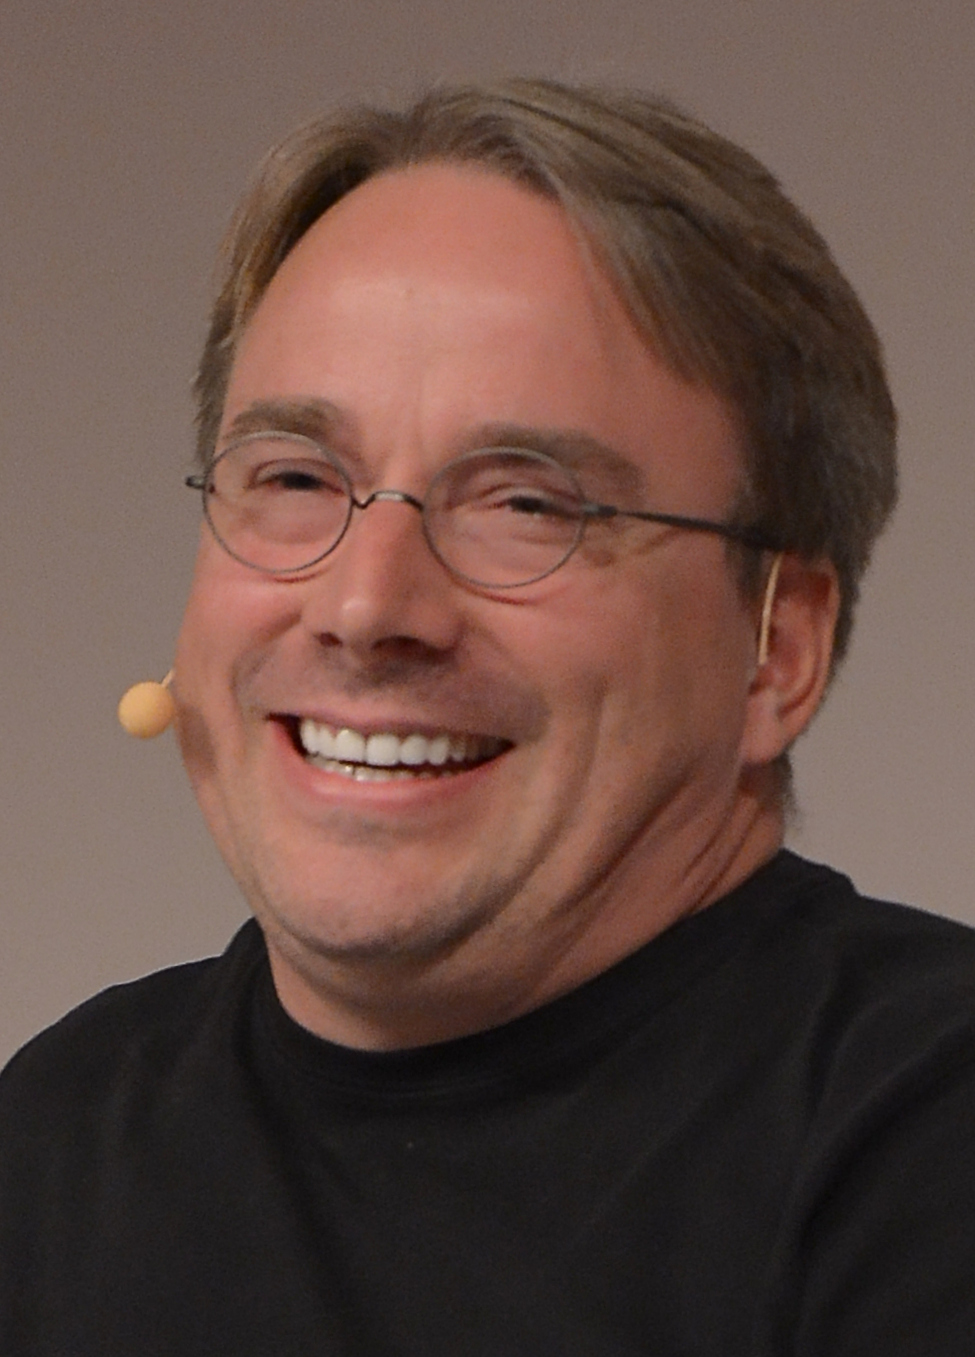
\includegraphics[width=0.5\textwidth]{figures/linus.jpg}
	  \caption{Linus Torvalds \textit{Source}: Krd/Von Sprat. License: CC BY-SA 4.0. \href{https://commons.wikimedia.org/wiki/File:LinuxCon_Europe_Linus_Torvalds_03.jpg}{https://commons.wikimedia.org}}
  \end{figure}  
    
  \end{column}
\end{columns}

\end{frame}

\section{What is version control?}

\begin{frame}{Local version control}
  \begin{figure}
	  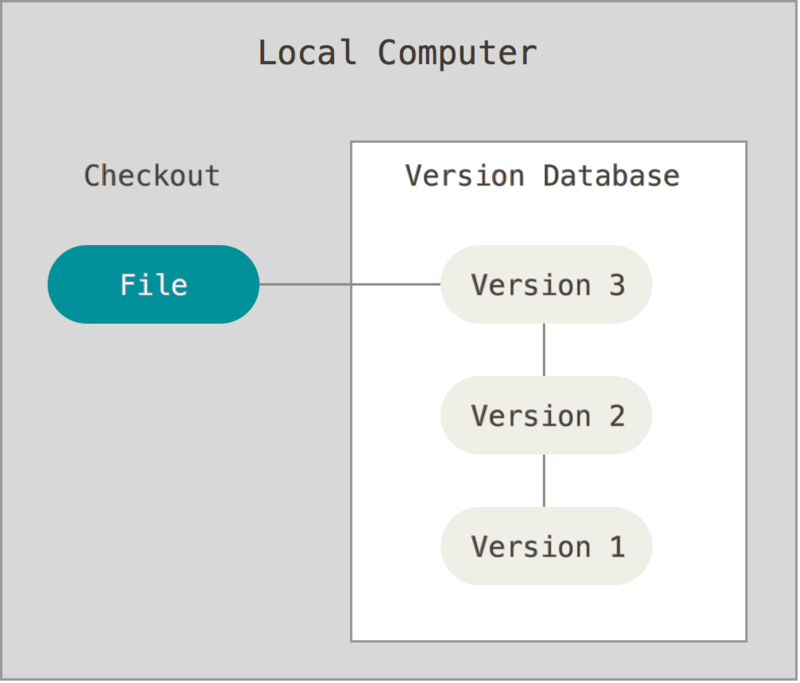
\includegraphics[width=0.6\textwidth]{figures/fig1_local.png}
	  \caption{Local version control \textit{Source}: Chacon \& Straub (2021), Figure 1.}
  \end{figure} 
\end{frame}

\begin{frame}{Centralized version control}
  \begin{figure}
	  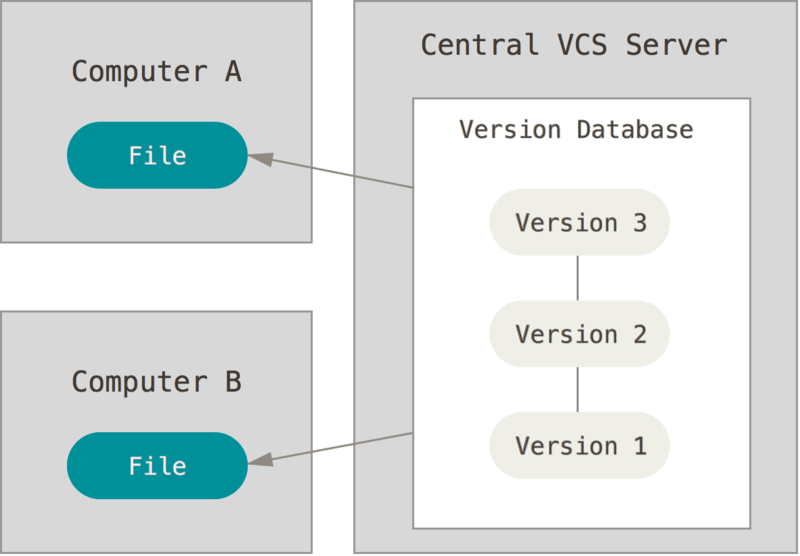
\includegraphics[width=0.7\textwidth]{figures/fig2_cvcs.png}
	  \caption{Centralized version control system (CVCS) \textit{Source}: Chacon \& Straub (2021), Figure 2.}
  \end{figure} 
\end{frame}

\begin{frame}{Distributed version control}
  \begin{figure}
	  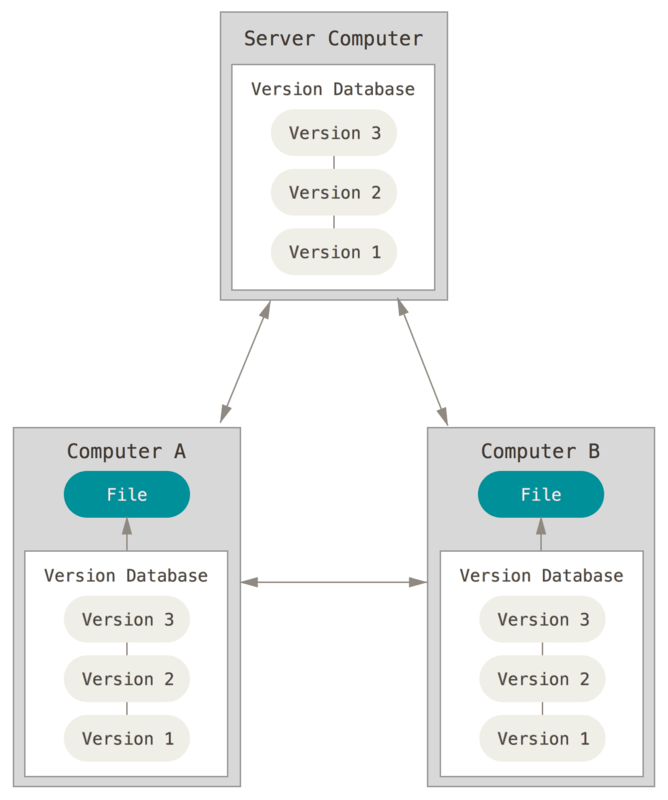
\includegraphics[width=0.5\textwidth]{figures/fig3_dvcs.png}
	  \caption{Distributed version control system (DVCS) \textit{Source}: Chacon \& Straub (2021), Figure 3.}
  \end{figure} 
\end{frame}


\section{What is Git?}

\begin{frame}{Snapshots}
  \begin{figure}
	  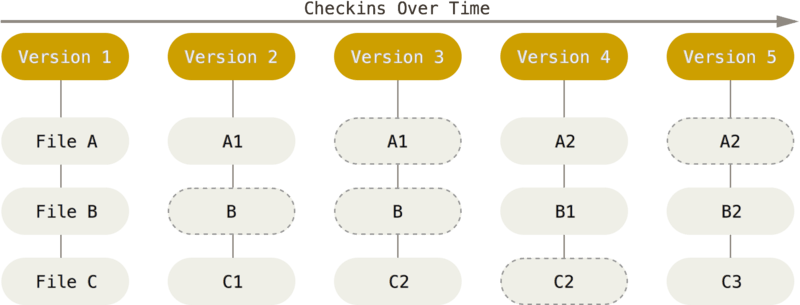
\includegraphics[width=0.8\textwidth]{figures/fig5_snapshots.png}
	  \caption{Git stores the version history of a project as a stream of snapshots over time. \textit{Source}: Chacon \& Straub (2021), Figure 5.}
  \end{figure} 
\end{frame}

\begin{frame}{The three states}
  \begin{figure}
	  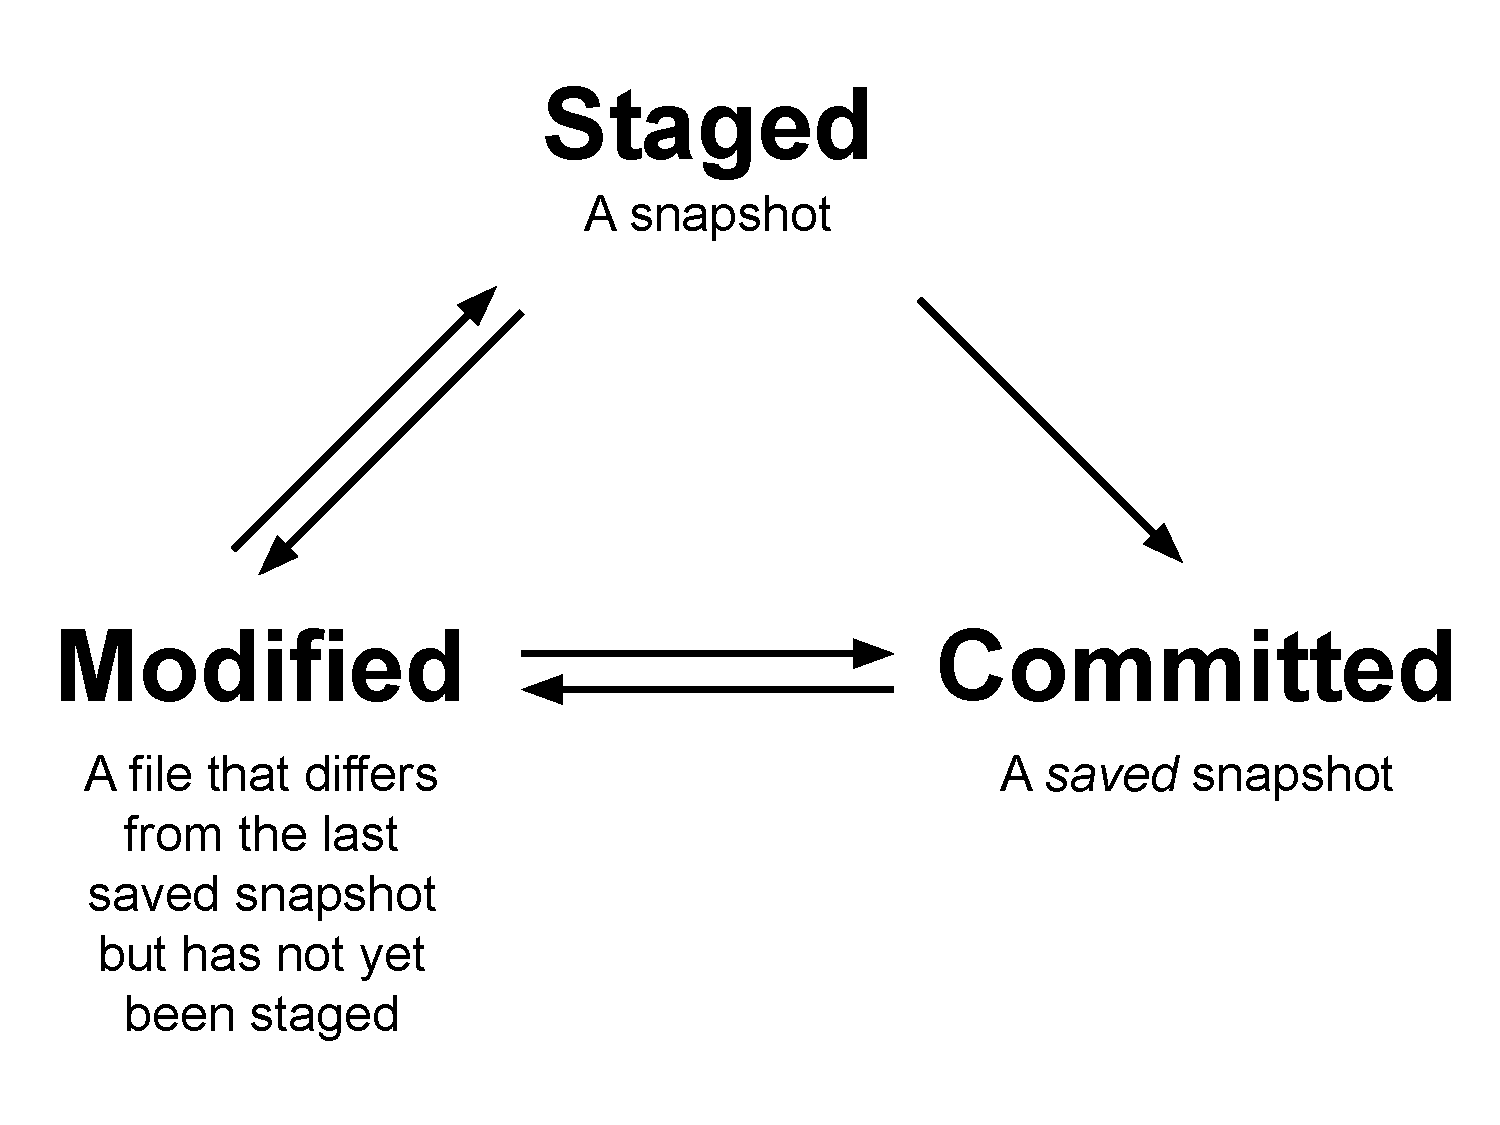
\includegraphics[width=0.8\textwidth]{figures/git_states.pdf}
	  \caption{In a git repository, a file can reside in three states: modified, staged, and committed}
  \end{figure} 
\end{frame}

\begin{frame}{The Git workflow}
  \begin{exampleblock}{The basic Git workflow goes something like this:}
    \begin{enumerate}
      \item You \textbf{modify} files in your working directory.
      \item You selectively \textbf{stage} just those changes you want to be part of your next commit.
      \item You do a \textbf{commit}, which takes the files as they are in the staging area and stores that snapshot permanently to your Git directory.
    \end{enumerate}
  \end{exampleblock}
  {\scriptsize Adapted from Chacon \& Straub (2021), Section 1.3.}
\end{frame}

\section{Git Setup}

\begin{frame}{Why using Git from the command line?}
  \begin{itemize}
    \item The only way to really learn the mechanics of Git. 
    \item Access to \textbf{all} Git functions.
    \item Easier to get help
  \end{itemize}
\end{frame}

\begin{frame}{Your identity}
  \begin{exampleblock}{Set your global user name and email address}
    \begin{semiverbatim}
      \item \$ git config --global user.name "John Doe"
      \item \$ git config --global user.email johndoe@example.com
    \end{semiverbatim}
  \end{exampleblock}
  \textit{Note}: Your email address is an integral part of your version history in Git. If you make your repository available, everyone will see your email address. Choose wisely!
\end{frame}

\begin{frame}{Other settings}
  By default, Git uses \textbf{Vim} as editor for certain operations. If you have installed \textbf{atom}, I would recommend using it as your default editor instead.  
  \begin{exampleblock}{Change your default editor}
    \begin{semiverbatim}
      \item \$ git config --global core.editor "atom --wait"
    \end{semiverbatim}
  \end{exampleblock}
  The default branch name on Git is \texttt{master}. I would recommend changing the default name to \texttt{main} (only possible from \texttt{git --version} 2.28 onwards). 
  \begin{exampleblock}{Change your default branch name}
    \begin{semiverbatim}
      \item \$ git config --global init.defaultBranch main
    \end{semiverbatim}
  \end{exampleblock}
\end{frame}

\begin{frame}{Viewing all your settings}
  \begin{exampleblock}{}
    \begin{semiverbatim}
      \item \$ git config --list
    \end{semiverbatim}
  \end{exampleblock}
  \begin{exampleblock}{}
    \begin{semiverbatim}
      \item user.email=philippe.joly@posteo.net
      \item user.name=Philippe Joly
      \item init.defaultbranch=main
      \item core.editor=atom --wait
    \end{semiverbatim}
  \end{exampleblock}
\end{frame}

\begin{frame}{Getting help}
  \begin{exampleblock}{Three equivalent ways to get the comprehensive manual page}
    \begin{semiverbatim}  
      \item \$ git help <verb>
      \item \$ git <verb> --help
      \item \$ man git-<verb>
    \end{semiverbatim}
  \end{exampleblock}
  \begin{exampleblock}{More concise “help” output }
    \begin{semiverbatim}  
      \item \$ git <verb> -h
    \end{semiverbatim}
  \end{exampleblock}
\end{frame}

\begin{frame}{What we have learned in this part of the workshop}
  \begin{itemize}
    \item The concepts behind a distributed version control system
    \item The three states a file can reside in inside Git
    \item The basic Git workflow
    \item Setting up your identity
    \item Other settings
    \item Getting help
  \end{itemize}
\end{frame}

\begin{frame}{Exercises}
  \begin{enumerate}
    \item Find the version of Git you are using with \texttt{git --version}.
    \item Set your global \texttt{user.name}.
    \item Set your global \texttt{user.email}.
    \item If you want, change your default \texttt{core.editor}.
    \item Set your default branch name to \texttt{main} (Git version $\geqslant$ 2.28).
    \item Examine all your settings. 
    \item Examine the concise help output for the \texttt{git config} command.
  \end{enumerate}
\end{frame}

\end{document}
